%%%%%%%%%%%%%%%%%%%%%%%%%%%%%%%%%%%%%%%%%
% Short Sectioned Assignment
% LaTeX Template
% Version 1.0 (5/5/12)
%
% This template has been downloaded from:
% http://www.LaTeXTemplates.com
%
% Original author:
% Frits Wenneker (http://www.howtotex.com)
%
% License:
% CC BY-NC-SA 3.0 (http://creativecommons.org/licenses/by-nc-sa/3.0/)
%
%%%%%%%%%%%%%%%%%%%%%%%%%%%%%%%%%%%%%%%%%

%----------------------------------------------------------------------------------------
%	PACKAGES AND OTHER DOCUMENT CONFIGURATIONS
%----------------------------------------------------------------------------------------

\documentclass[paper=a4, margin=10mm, fontsize=11pt]{scrartcl} % A4 paper and 11pt font size

\usepackage[T1]{fontenc} % Use 8-bit encoding that has 256 glyphs
\usepackage{fourier} % Use the Adobe Utopia font for the document - comment this line to return to the LaTeX default
\usepackage[english]{babel} % English language/hyphenation
\usepackage{amsmath,amsfonts,amsthm,amssymb} % Math packages

\usepackage{lipsum} % Used for inserting dummy 'Lorem ipsum' text into the template

\usepackage{sectsty} % Allows customizing section commands
\allsectionsfont{\centering \normalfont\scshape} % Make all sections centered, the default font and small caps

\usepackage{fancyhdr} % Custom headers and footers

% my packages
\usepackage{commath}
\usepackage{mathtools}
\usepackage{graphicx}
\usepackage{algorithm}
\usepackage[]{algpseudocode}
\DeclarePairedDelimiter{\ceil}{\lceil}{\rceil}
\usepackage{pgfplots}
\pgfplotsset{compat=newest}
\usepackage{hyperref}
\usepackage{enumitem}
\usepackage{caption}
\usepackage{subcaption}
\usepackage{multirow}
\usepackage{tkz-graph}
\usepackage{adjustbox}
\usepackage{cancel}
\usepackage[percent]{overpic}

\newlist{filedescription}{description}{2}
\setlist[filedescription]{font=\normalfont\normalcolor\bfseries\itshape}

\newlist{paramdescription}{description}{1}
\setlist[paramdescription]{font=\normalfont\normalcolor\itshape}

\pagestyle{fancyplain} % Makes all pages in the document conform to the custom headers and footers
\fancyhead{} % No page header - if you want one, create it in the same way as the footers below
\fancyfoot[L]{} % Empty left footer
\fancyfoot[C]{} % Empty center footer
\fancyfoot[R]{\thepage} % Page numbering for right footer
\renewcommand{\headrulewidth}{0pt} % Remove header underlines
\renewcommand{\footrulewidth}{0pt} % Remove footer underlines
\setlength{\headheight}{13.6pt} % Customize the height of the header

\numberwithin{equation}{section} % Number equations within sections (i.e. 1.1, 1.2, 2.1, 2.2 instead of 1, 2, 3, 4)
\numberwithin{figure}{section} % Number figures within sections (i.e. 1.1, 1.2, 2.1, 2.2 instead of 1, 2, 3, 4)
\numberwithin{table}{section} % Number tables within sections (i.e. 1.1, 1.2, 2.1, 2.2 instead of 1, 2, 3, 4)

\setlength\parindent{0pt} % Removes all indentation from paragraphs - comment this line for an assignment with lots of text

% new commands
\newcommand{\filename}[1]{\textbf{\textit{#1}}}
\newcommand{\funcname}[1]{\textbf{#1}}
\newcommand{\inv}{^{\raisebox{.2ex}{$\scriptscriptstyle-1$}}}
\renewcommand{\vec}[1]{\mathbf{#1}}

\makeatletter
\renewcommand*\env@matrix[1][*\c@MaxMatrixCols c]{%
  \hskip -\arraycolsep
  \let\@ifnextchar\new@ifnextchar
  \array{#1}}
\makeatother

\makeatletter
\def\BState{\State\hskip-\ALG@thistlm}
\makeatother

\DeclareMathAlphabet{\mathcal}{OMS}{cmsy}{m}{n}
\DeclareMathOperator*{\argmin}{arg\,min} % Jan Hlavacek

\newtheorem{theorem}{Theorem}
\newtheorem{definition}{Definition}

%----------------------------------------------------------------------------------------
%	TITLE SECTION
%----------------------------------------------------------------------------------------

\newcommand{\horrule}[1]{\rule{\linewidth}{#1}} % Create horizontal rule command with 1 argument of height

\title{	
\normalfont \normalsize 
\textsc{Recursive Estimation Spring 2017, ETH Zurich} \\ [25pt] % Your university, school and/or department name(s)
\horrule{0.5pt} \\[0.4cm] % Thin top horizontal rule
\huge Extended Kalman Filter \\ for Tracking a Three-Wheeled Robot \\ % The assignment title
\horrule{2pt} \\[0.5cm] % Thick bottom horizontal rule
}

\author{Dong Ho Kang and Jaeyoung Lim} % Your name

\date{\normalsize June 7, 2017} % Today's date or a custom date

\begin{document}

\maketitle % Print the title

%----------------------------------------------------------------------------------------
%	HISTOGRAM
%----------------------------------------------------------------------------------------

\graphicspath{{figures/}} 

\begin{itemize}
	\item $Q_{v1} = 0.01 \text{(rad/s)}^2/\text{Hz}$

\begin{figure}[H]
\centering
\noindent\makebox[\textwidth]{
  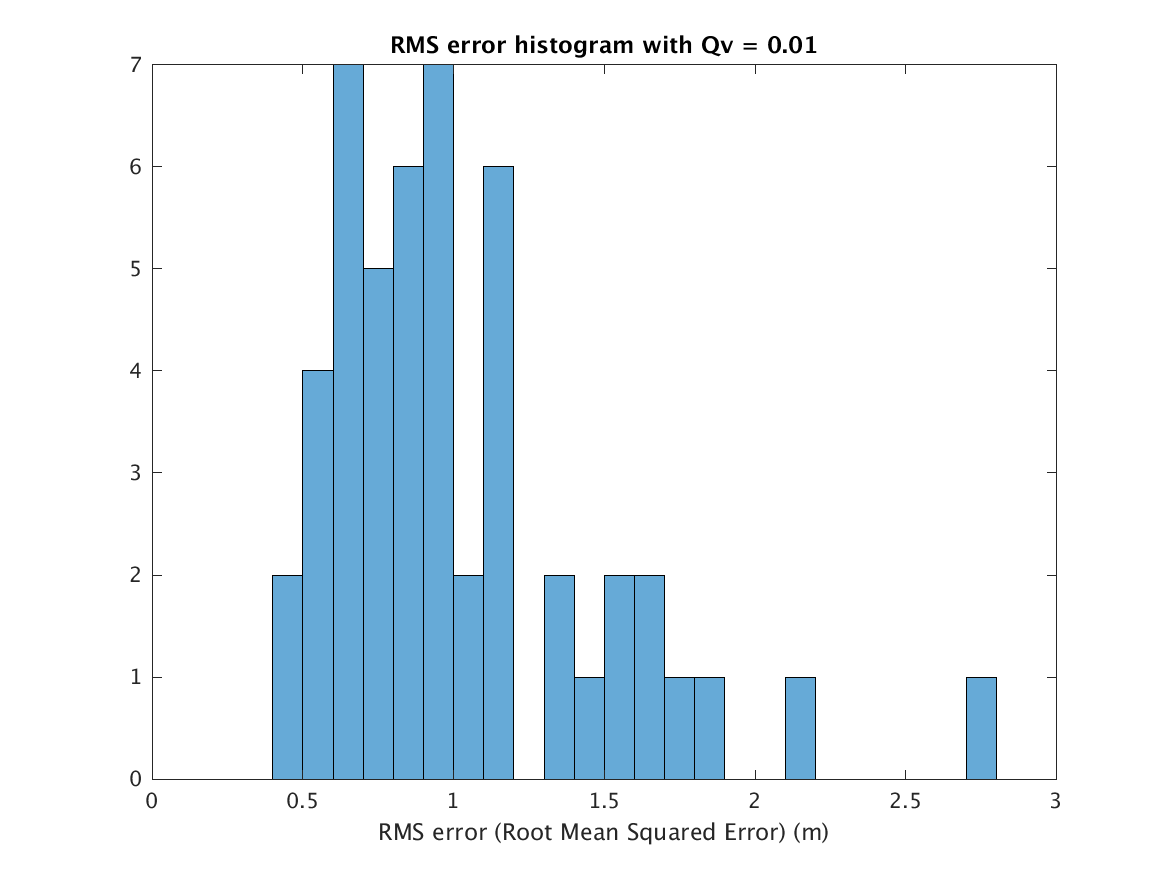
\includegraphics[width=0.9\textwidth]{hist1.png}
}
\end{figure}
	
	\item $Q_{v2} = 0.1 \text{(rad/s)}^2/\text{Hz}$

\begin{figure}[H]
\centering
\noindent\makebox[\textwidth]{
  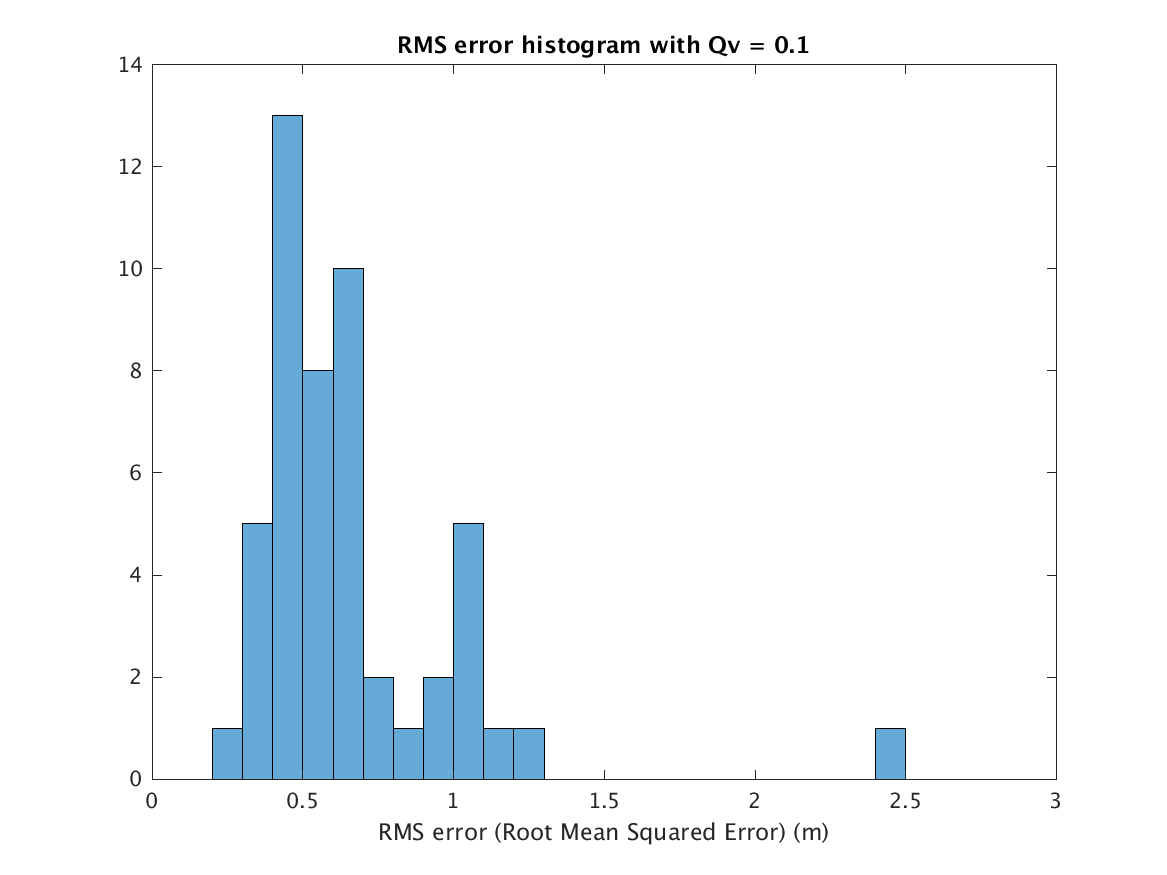
\includegraphics[width=0.9\textwidth]{hist2.png}
}
\end{figure}
	
	\item $Q_{v3} = 1.0 \text{(rad/s)}^2/\text{Hz}$

\begin{figure}[H]
\centering
\noindent\makebox[\textwidth]{
  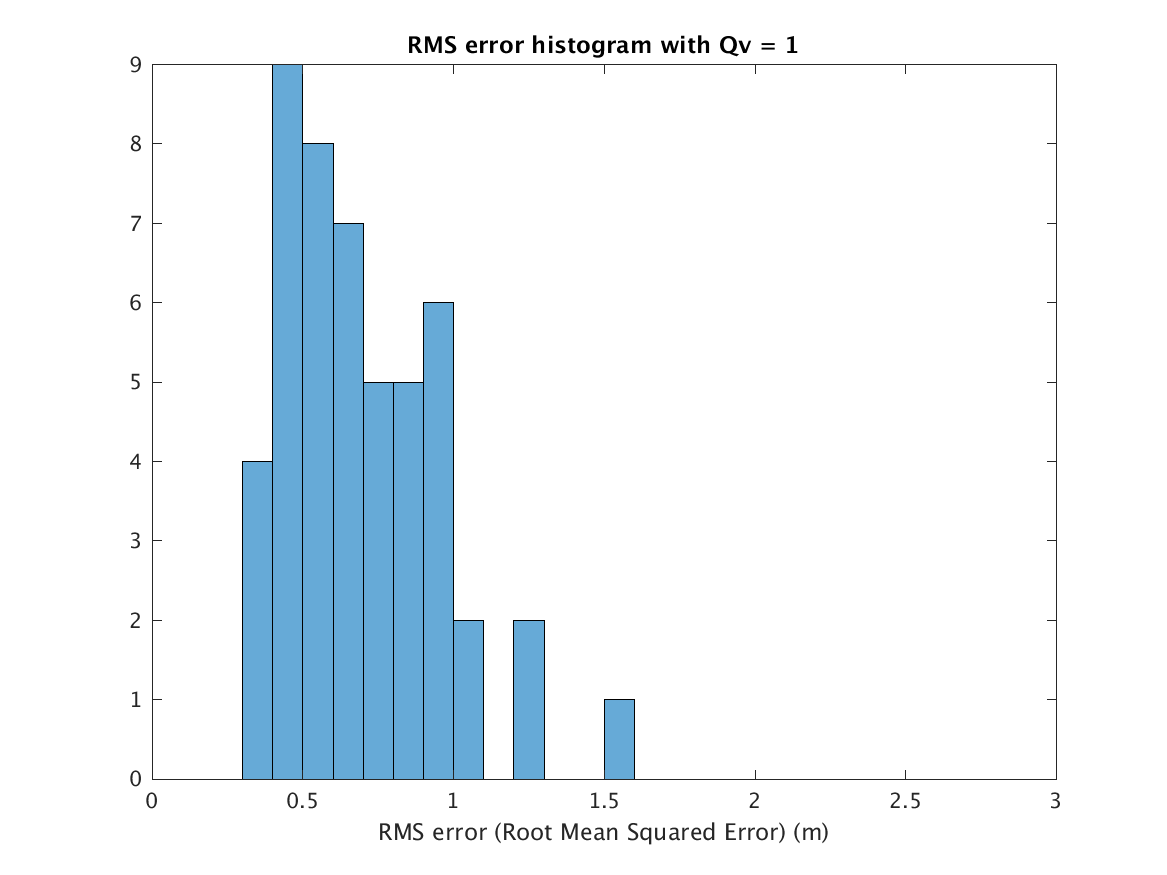
\includegraphics[width=0.9\textwidth]{hist3.png}
}
\end{figure}

\end{itemize}


\begin{figure}[H]
	\caption{batman.jpg \label{fig:batman}}
	\centering
	\begin{subfigure}[b]{0.3\textwidth}
		\noindent\makebox[\textwidth]{
		  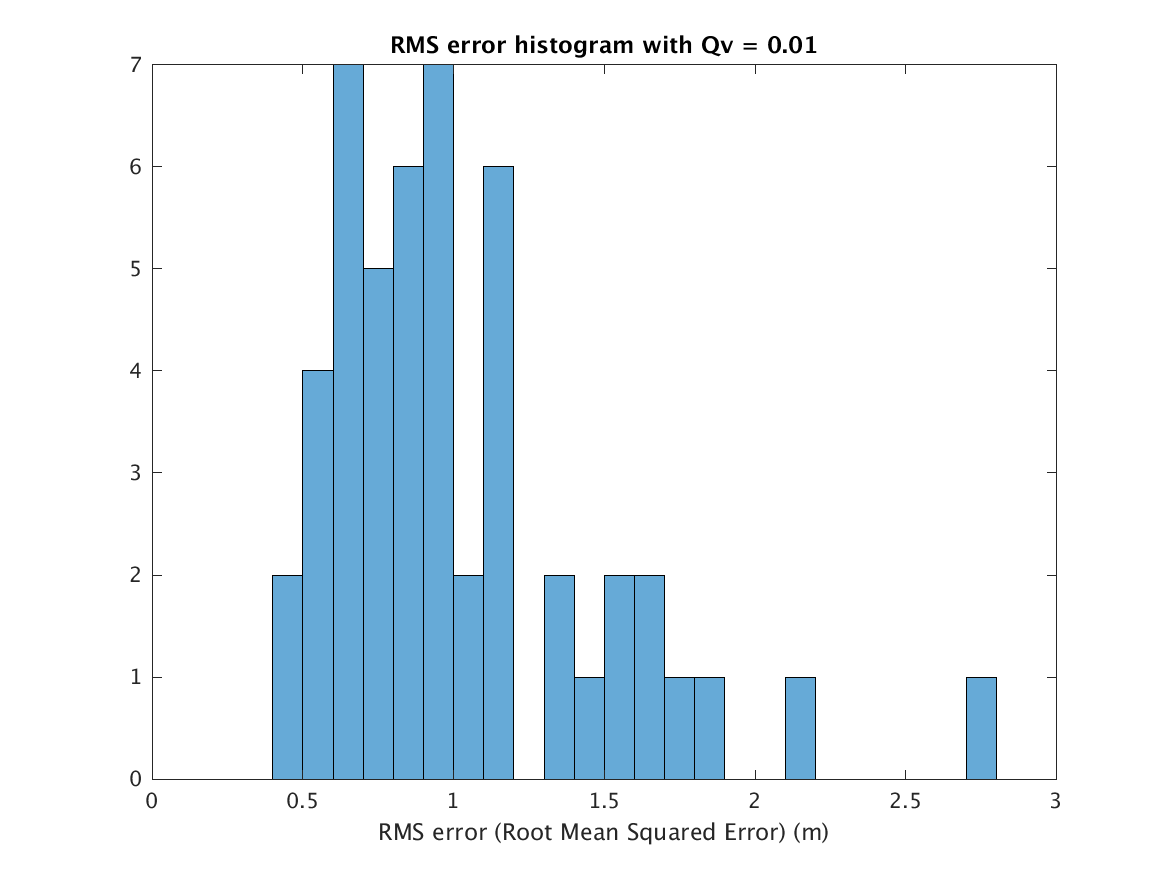
\includegraphics[width=\textwidth]{hist1.png}
		}
	\caption{batman.jpg \label{fig:vaorig}}
	\end{subfigure}
	\begin{subfigure}[b]{0.3\textwidth}
		\noindent\makebox[\textwidth]{
		  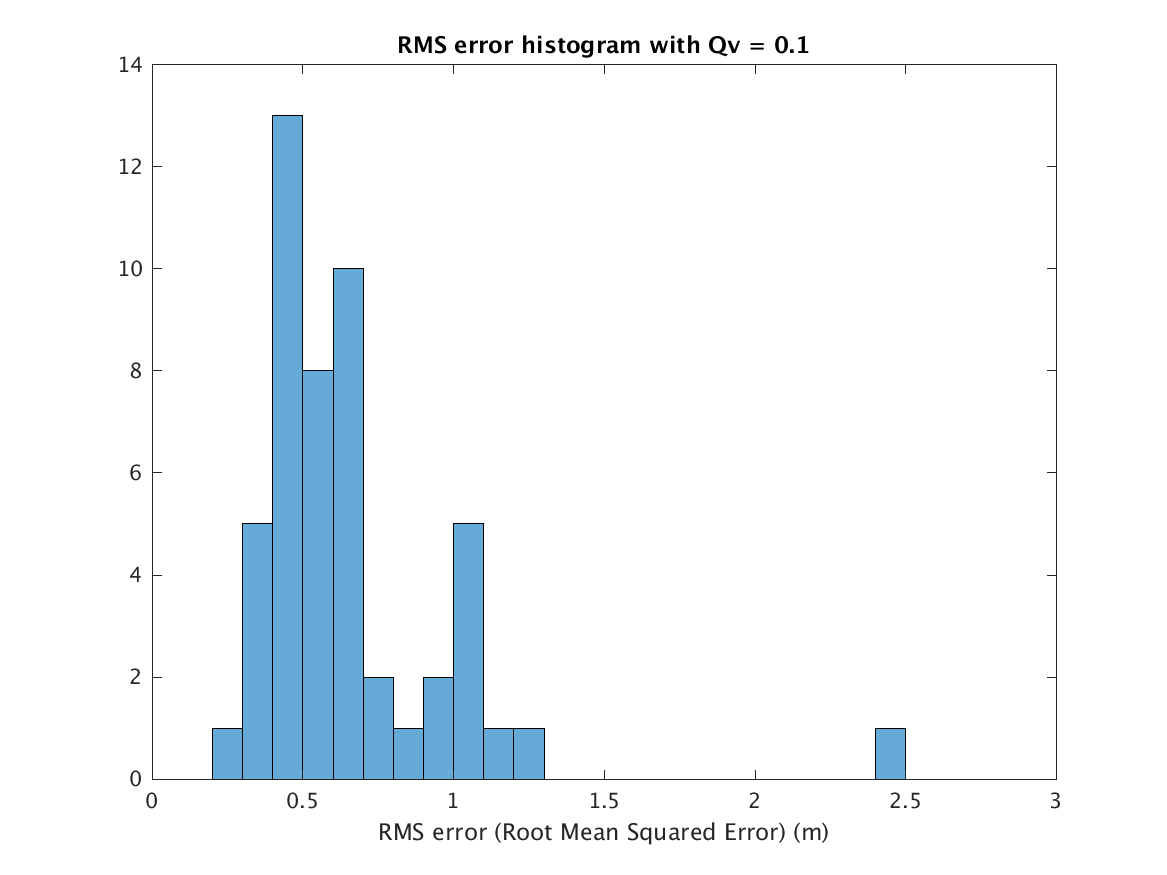
\includegraphics[width=\textwidth]{hist2.png}
		}
	\caption{Scribbles for the color histogram \label{fig:vadenoised}}
	\end{subfigure}
	\begin{subfigure}[b]{0.3\textwidth}
		\noindent\makebox[\textwidth]{
		  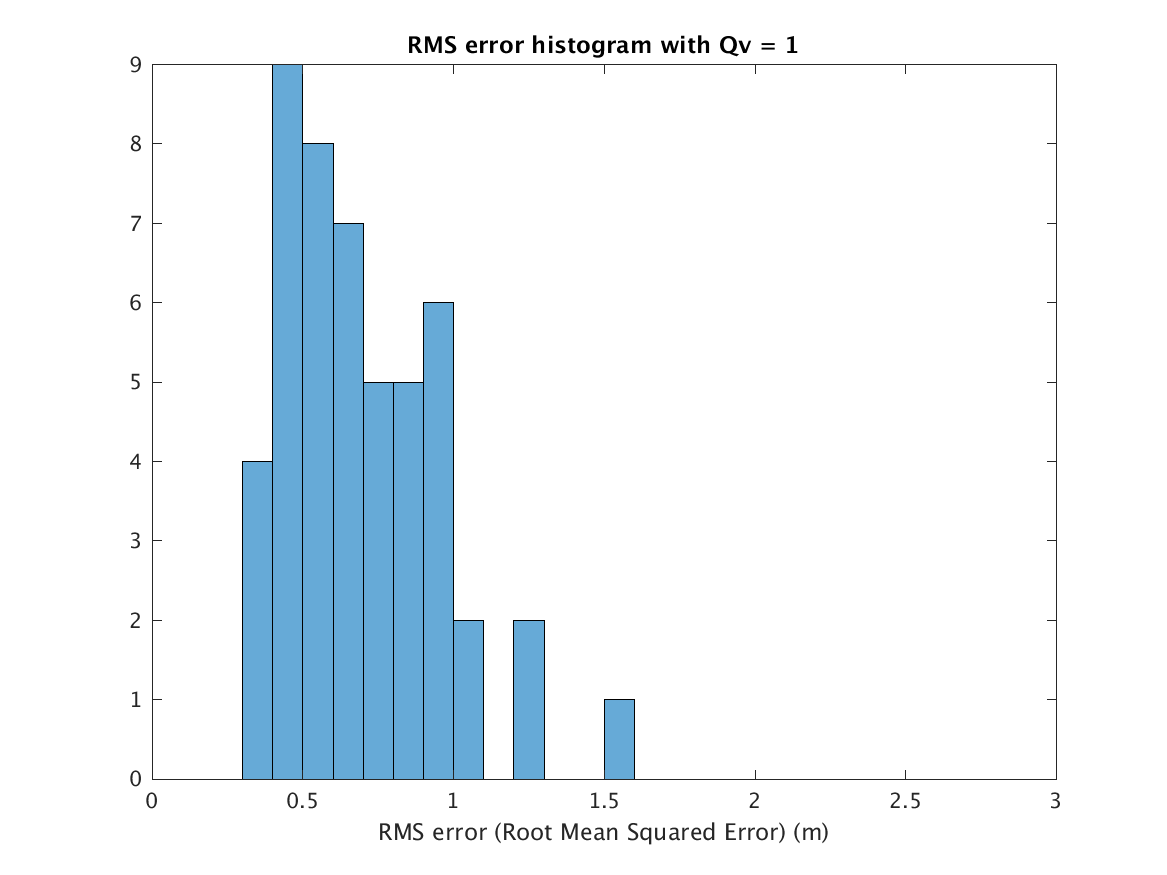
\includegraphics[width=\textwidth]{hist3.png}
		}
	\caption{Scribbles for the color histogram \label{fig:vadenoised}}
	\end{subfigure}
\end{figure}


\end{document}